% !TEX root = ../main.tex
% Chapter Experimental setup

\chapter{Experimental setup} % Main chapter title

\label{Chapter3} % Change X to a consecutive number; for referencing this chapter elsewhere, use \ref{ChapterX}

This chapter reviews the different experiments undertaken during this thesis. The goal of these experiments is to measure the effectiveness of more complex models against simple ones, different preprocessing strategies and the computational performance between different GPUs. All models are trained with the Cornell Movie Dialogs corpus.

\section{Cornell Movie Dialogs corpus}
The Cornell Movie Dialogs corpus \citep{cornell} is constructed from raw movie scripts. It has 220,579 conversational exchanges between 10,292 pairs of movie characters involving 9,035 characters from 617 movies. Here are some examples from the corpus.

\begin{center}
    ``You have my word.  As a gentleman'' - ``You're sweet.''\\
    ``There.'' - ``Where?''\\
    ``Gosh, if only we could find Kat a boyfriend...'' - ``Let me see what I can do.''
\end{center}

The texts have very different lengths. Table~\ref{tab:stats-cornell} shows some statistics of text lengths and Figure~\ref{fig:hist-cornell-senteces-length} illustrates the conversations' length distribution. The large majority of conversations does not exceed 15 words.

\begin{table}
    \centering
    \caption[Statistics sentence corpus length]{Statistics of sentences' lengths for Cornell Movie Dialogs corpus. All measures are letter-wise and not word-wise, except ``Utterances'' that simply represent the number of conversations in the dataset.}
    \label{tab:stats-cornell}
    \begin{tabular}{c|ccccccc}
        \toprule
        \tabhead{Utterances} & \tabhead{Mean} & \tabhead{Min} & \tabhead{Max} & \tabhead{Std} & \tabhead{25\%} & \tabhead{50\%} & \tabhead{75\%}\\
        \midrule
        304713 & 55.32 & 1 & 3046 & 64.09 & 19 & 35 & 69\\
        \bottomrule
    \end{tabular}
\end{table}

\begin{figure}
    \centering
    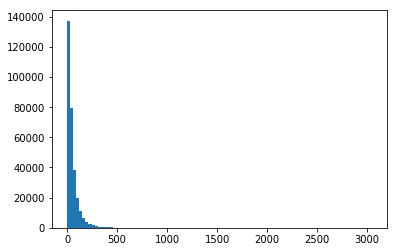
\includegraphics[width=.8\textwidth]{hist_cornell_sentences_length}
    \decoRule
    \caption[Conversations length distribution]{Conversations length distribution. The average word length in English is about five letters~\citep{wolframlanguage}, thus the large majority of the conversations does not exceed 15 words. X-axis represents the sentences lengths (letter-wised) and Y-axis represents the number of sentences.}
    \label{fig:hist-cornell-senteces-length}
\end{figure}

\section{Experiments model architecture}
The general purpose of this chatbot is to learn how to converse with other humans based on the movie dialogs. The model's architecture follows the Neural Machine Translation (NMT) model.
Instead of translating from a language to another, the model ``translates'' the question into an answer, since the input and output have the same form in both cases.

Since dialogs in movies are open-domain conversations, just splitting the dataset into an 80-10-10 division (80\% training set, 10\% development set, 10\% test set, \citet{jurafsky2014speech})to train models might not work well. Thus, the idea is to find a closer domain even in this context by trying to train the model to act like one of the movie character. To ensure that the training does not suffer from the lack of data, the character is chosen based on the number of conversations he is involved into. Table~\ref{tab:char-cornell} shows the five most present characters.

\begin{table}
    \caption[Character presence analysis]{Character presence analysis within the Cornell Movie Dialogs corpus presenting the five most present characters.}
    \label{tab:char-cornell}
    \centering
    \begin{tabular}{llllll}
        \toprule
        & \tabhead{Jack} & \tabhead{Joe} & \tabhead{George} & \tabhead{Frank} & \tabhead{Nick}\\
        \midrule
        \tabhead{Utterances} & 3032 & 1897 & 1748 & 1537 & 1484\\
        \bottomrule
    \end{tabular}
\end{table}

In all of the different runs, the training is done in two phases, namely the training, based on all of the conversations, and the fine-tuning, based only on the conversations where the chosen character is answering. Other features like the gender of the character speaking first might lead to better results.


\section{Data preprocessing}
Raw string sentence is preprocessed in order to give the encoder, and the decoder, a tokenized sequence. There are different steps to prepare data for training and these steps are illustrated in Figure~\ref{fig:preprocess}. First, the raw sentence is tokenized to separate words and punctuation, the casing is not changed because it carries different information (e.g. start of sentence).

\begin{figure}
    \centering
    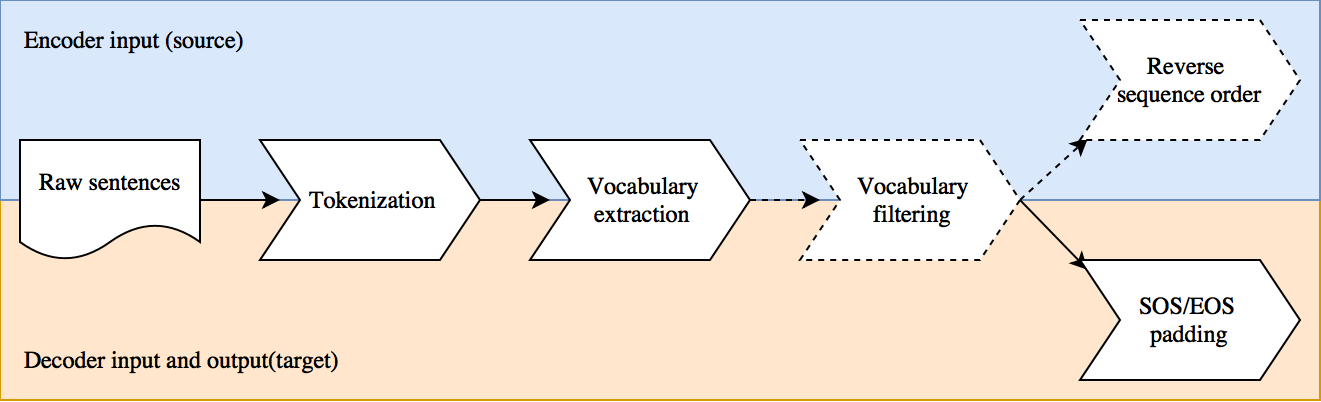
\includegraphics[width=\textwidth]{preprocess}
    \decoRule
    \caption[Preprocessing steps in NMT]{Preprocessing steps in an NMT model. Shapes with discontinued line refer to optional steps.}
    \label{fig:preprocess}
\end{figure}

Secondly, from the tokenized sentences, the preprocessor extracts the vocabulary (i.e. all of the tokens with the number of times it appears). Table~\ref{tab:src-vocab} summarizes source vocabulary and Table~\ref{tab:tgt-vocab} summarizes target vocabulary.
Published work shows that people tend to limit the vocabulary. For example, \citet{1508.04025}, with a dataset of 4.5M sentence pairs (20 times the size of Cornell Movies Dialogs corpus), the vocabulary was limited to the 50K most frequent words. Additionally, in \citet{1506.06714}, with a dataset of 12M sentences, the vocabulary was also limited to the 50K most frequent words.
Table~\ref{tab:reduce-vocab} illustrates how both vocabularies can be reduced by using a threshold on word counts and only keep the most frequent ones.
In~\citet{1506.05869}, two different datasets were used. The first dataset contained 33M sentences and the vocabulary was limited to 20K words, and in the second dataset, composed of 88M sentences, the vocabulary was limited to 100K words.

\begin{table}
    \centering
    \caption[Source vocabulary analysis]{Source vocabulary analysis. The number of unique words:~\num{64839}. For example, it only takes \num{12603} words (\num{19.43}\% of the vocabulary) to reach \num{97}\% of the source sentences word count.}
    \label{tab:src-vocab}
    \begin{tabular}{rrr|r}
        \toprule
        \tabhead{Total count \%} & \tabhead{Unique words} & \tabhead{Vocabulary \%} & \tabhead{Current count value}\\
        \midrule
        \num{90.0} & \num{1974} & \num{3.04} & \num{82}\\
        \num{97.0} & \num{12603} & \num{19.43} & \num{7}\\
        \num{98.0} & \num{19259} & \num{29.70} & \num{4}\\
        \num{99.0} & \num{32910} & \num{50.76} & \num{2}\\
        \num{99.9} & \num{61584} & \num{94.98} & \num{1}\\
        \bottomrule
    \end{tabular}
\end{table}

\begin{table}
    \centering
    \caption[Target vocabulary analysis]{Target vocabulary analysis. Number of unique words:~\num{65875}}
    \label{tab:tgt-vocab}
    \begin{tabular}{rrr|r}
        \toprule
        \tabhead{Total count \%} & \tabhead{Unique words} & \tabhead{Vocabulary \%} & \tabhead{Current count value}\\
        \midrule
        \num{90.0} & \num{1942} & \num{2.94} & \num{86}\\
        \num{97.0} & \num{12577} & \num{19.09} & \num{7}\\
        \num{98.0} & \num{19321} & \num{29.33} & \num{4}\\
        \num{99.0} & \num{33215} & \num{50.42} & \num{2}\\
        \num{99.9} & \num{62520} & \num{94.90} & \num{1}\\
        \bottomrule
    \end{tabular}
\end{table}

\begin{table}
    \centering
    \caption[Vocabulary reduction]{Limiting the vocabulary size based on the word counts.}
    \label{tab:reduce-vocab}
    \begin{tabular}{rrrr}
        \toprule
        \tabhead{Min count} & \tabhead{Unique words} & \tabhead{Vocabulary \%} & \tabhead{Total count \%}\\
        \midrule
        \multicolumn{4}{l}{\textit{Source vocabulary}}\\
        \num{3} & \num{24347} & \num{37.55} & \num{98.47}\\
        \num{5} & \num{16456} & \num{25.38} & \num{97.66}\\
        \num{10} & \num{9881} & \num{15.24} & \num{96.34}\\
        \hline
        \multicolumn{4}{l}{\textit{Target vocabulary}}\\
        \num{3} & \num{24736} & \num{37.37} & \num{98.49}\\
        \num{5} & \num{16724} & \num{25.39} & \num{97.69}\\
        \num{10} & \num{9947} & \num{15.10} & \num{96.38}\\
        \bottomrule
    \end{tabular}
\end{table}

The final step of the preprocessing is different from the source and target set. Source sentences can be reversed, word-wise, to improve performance as mentioned in \citet{1409.3215}.
The last encoder's hidden state is the beginning of the sentence and it allows the decoder to be closer to the start of the sequence.
Target sentences need to be padded with Start-Of-Sequence (SOS) and End-Of-Sequence (EOS) tokens to let the decoder know when the sequence starts and stops.

The source and target vocabularies present similar statistics because of the fact that most of the conversations present in the corpus have multiple turns. Thus, for example, conversation \code{[A, B, C, D]} is fed into the training set as \code{[(A, B), (B, C), (C, D)]} which makes \code{[B, C]} appear in both source and target sets.

\section{Tensorflow and Neural Machine Translation tutorial}
The models' training has been done using the NMT tutorial script by~\citet{tensorflow.nmt}. The authors use the Tensorflow~\citep{tensorflow2015-whitepaper} open-source library made ``\textit{for numerical computation using data flow graphs}''. Tensorflow simplifies development tasks in a machine-learning project. The developer creates his model as a graph, where nodes are operations and edges are matrices (tensors). From this graph definition of the mathematical model, Tensorflow automatically calculates the gradients and the derivatives needed for backpropagation.
Another advantage to use Tensorflow is that it runs on either CPUs or GPUs without changing a line of code. The same code is used when the engineer works locally on its machine and when the model is trained on servers with dedicated GPU cards.

The NMT tutorial script was written to let people create and train an NMT model without having to spend time coding and debugging the algorithms. The script is part of a 5 years long Ph.D. thesis \citep{nmt-phd}. The script has 65 different arguments, detailed in Appendix~\ref{AppendixA}, going from the type of RNN to the attention's type of architecture.

\section{Infrastructures}
The server used in this thesis is hosted on a GPU accelerated cloud platform, Paperspace\footnote{https://www.paperspace.com/} with pre-configured flavors for machine learning applications. The machine used for all experiments is the ``\textit{GPU+}'' flavor configured with 30GB RAM, 8 CPU cores and a dedicated NVIDIA Quadro M4000. Only one training was performed also on another machine to analyze if the cost of a more expensive flavor is worth the time saved.
The more expensive is actually the most expensive one proposed by Paperspace with a dedicated last-generation NVIDIA Tesla V100, Volta generation. Table~\ref{tab:paperspace-flavors} summarizes the differences between the two flavors. The ``\textit{V100}'' flavor costs almost 6 times more than the other flavor.

\begin{table}
    \centering
    \caption[Paperspace flavors]{Paperspace dedicated GPU flavors differences.}
    \label{tab:paperspace-flavors}
    \begin{tabular}{lllllll}
        \toprule
        \tabhead{Flavor} & \tabhead{Generation} & \tabhead{VRAM} & \tabhead{Bandwith} & \tabhead{Performance} & \tabhead{Price}\\
        \midrule
        GPU+ & Maxwell & 8 GB & 192 GB/s & 2.6 teraFLOPS & \$0.40 per hour\\
        V100 & Volta & 16 GB & 900 GB/s & 112 teraFLOPS & \$2.30 per hour\\
        \bottomrule
    \end{tabular}
\end{table}
